\documentclass[12pt]{article}

\usepackage[utf8]{inputenc}
\usepackage{amsmath}
\usepackage{amsfonts}
\usepackage{amssymb}
\usepackage{graphicx}
\usepackage{ulem} 

\usepackage[export]{adjustbox}
\usepackage{subfig}

\usepackage{float}


\begin{document}
% Title
\title{March Update}
\maketitle

% %% INTRO
\section{Introduction}
Our primary goal during the first phase of this project has been to measure the influence of pseudoproxy information on the prior. To this end we would like to test for, and quantify, significant differences between the prior and the posterior ensemble. Our work so far has revolved around trying to answer the following three questions:


\begin{enumerate}
\item Is the prior significantly different from the ensemble?
\item If so, where is it different?
\item And if so, by how much is it different?
\end{enumerate}

%%% DATA
\section{Data}
Our analysis, and this report, have been updated to use the latest reconstructions from February. This consists of 998 $96\times144$ prior ensembles and 100 $96\times144$ ensemble member fields observed over 1001 time points. So far we have only considered in detail a small subset of the time points for testing and illustration.

\section{Methods}
We assume that each random field, the prior and the ensemble members, are noisy observations of smooth 2-dimensional functions. In doing so, we simplify our testing and measurement problem from comparing random fields to comparing smooth functions. 

\subsection{Basis function smoothing}
In order to translate from random fields to smooth functions we first need to smooth the data by representing each field as a linear combination of basis functions. We chose to use the bisquare basis since they're multiresolutional, computationally efficient, and each represent distinct regions of the map\cite{cressie08}. The bisquare basis is defined by:

$$ f_{u_l}(s) = \bigg(1 -  \frac{||s - u_l||^2}{r^2}\bigg)^2  1_{(||s - u_l|| < r)} $$

Where $u_l$ is the center of the $l^{th}$ basis, $r$ = $1.5\min_{i, j}(||u_i - u_j||)$  $ \forall	i, j \leq n$, and $s$ is any spatial location.  We can then approximate each field $g$ with a linear combination of $n$ basis functions:

$$ g(s)  = \sum_{i=1}^{n} \beta_i f_{u_i}(s)$$

The coefficients are estimated via OLS and the number of basis functions is selected by finding the representation which minimizes the Bayesian Information Criterion (BIC). BIC is a model selection criteria that penalizes the model's log-likelihood based on the number of basis functions to help prevent overfitting. 

Since the basis functions are the same for each random field, the coefficients form a unique, low dimensional, representation. Analysis on the coefficients is therefore equivalent to analysis on the field itself so our analysis below is all based on the coefficients. 

\subsection{Basis function selection}
To find an appropriate number of basis functions we considered both the MSE and the BIC\cite{Schwarz78} of our OLS estimated approximate field. A regularly spaced grid of 510 basis functions was found to minimize the BIC while maintaining a relatively small MSE. To gauge the sensitivity of our results against the number of basis functions we also looked at regularly spaced grids of 150, 240, and 375 basis functions. The grids were constructed by placing basis centers at the Cartesian product of a specified number of latitude and longitude points. For instance the 510 basis was constructed from the Cartesian product of 17 evenly spaced latitude points and 30 evenly spaced longitude points. 

\begin{figure}[H]
    \hspace{-2.5cm}\subfloat{{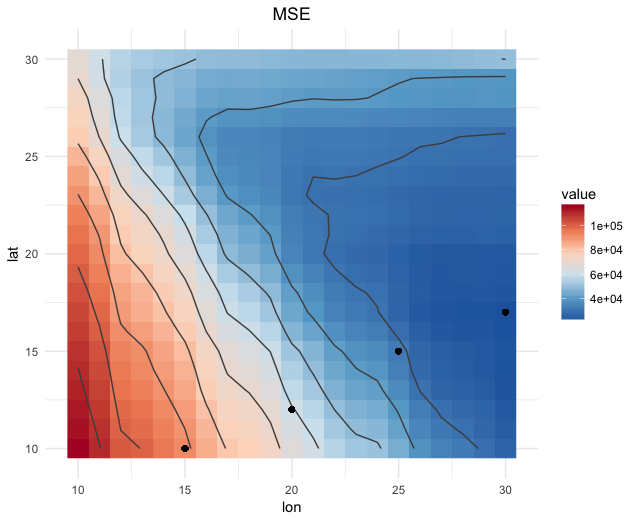
\includegraphics[width=0.7\textwidth]{../plots/Mse_basis.png}}}
    \subfloat{{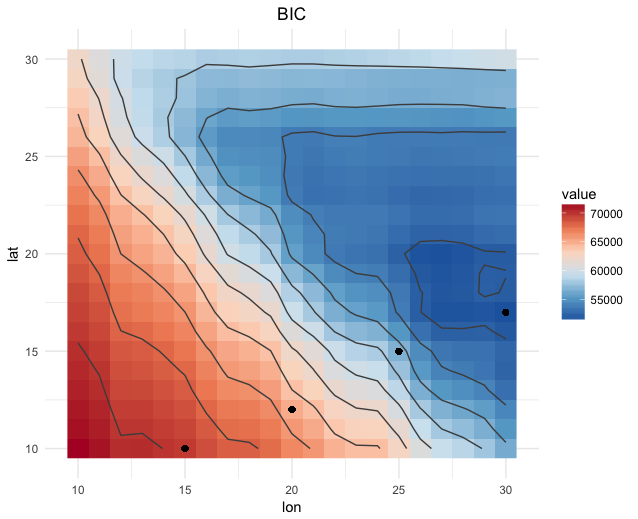
\includegraphics[width=0.7\textwidth]{../plots/Bic_basis.png}}}
    \caption{Basis Function Selection}
    \label{fig:basis}
\end{figure}


\subsection{Extremal Depth}
To test whether the prior resides within the ensemble we borrow a functional data depth technique called Extremal Depth. Essentially, Extremal Depth measures how ``deeply'' a function (the prior) sits within a set of other functions (the ensemble). ED ranges from 0 to 1 with higher values indicating deeper functions. An ED of 1 is considered the median\cite{naveen15}.

\subsection{Hypothesis Tests}
ED allows for the construction of central regions which, like confidence intervals, can be used to test hypothesis. One very nice property of ED is that, $1 - ED(prior)$, gives the $\alpha$ level of the smallest central region that contains the prior. In other words  $ED(prior)$ is the \textit{p} value\cite{naveen15}. of the following test:

\begin{center}
$ H_0:$ The prior comes from the same process as the ensemble

$ H_A:$ The prior does not come from the same process as the ensemble
\end{center}

\section{Results}

\subsection{Hypothesis Tests}
First we found the  \textit{p} values from the Extremal Depth of the prior with respect to the ensemble at each time point. \sout{In the vast majority of cases the \textit{p} value was found to be 0, indicating that the prior is significantly different from the ensemble}. One possible reason for this is because ED rejects $H_0$ if even a single prior basis coefficient is outside the range spanned by the ensemble's basis coefficients. Since the coefficients tend to be very close to each other, it's quite likely there will be at least one prior coefficient outside the range of the ensemble's.

To give a more informative presentation of the difference between the prior and ensembles, we plotted how far the prior was outside either the upper or lower limit of the $95\%$ central region for each coefficient. This gives a new vector of coefficients which represents a spatial field of the difference between the prior and the ensemble as a whole.

\subsection{Different numbers of basis functions}
Before examining specific time points in detail we wanted to see how sensitive both the Extremal depth tests and the ``difference fields'' were to an increasing number of basis functions. We found the Extremal Depth, central regions, and differences fields for the prior at time 400 for 150, 240, 375, and 510 basis functions. While all of the ED tests gave a \textit{p}  value of 0, the following plots show that the difference fields can be quite dissimilar.

\begin{figure}[H]

  \hspace{-2.5cm}\subfloat{%
    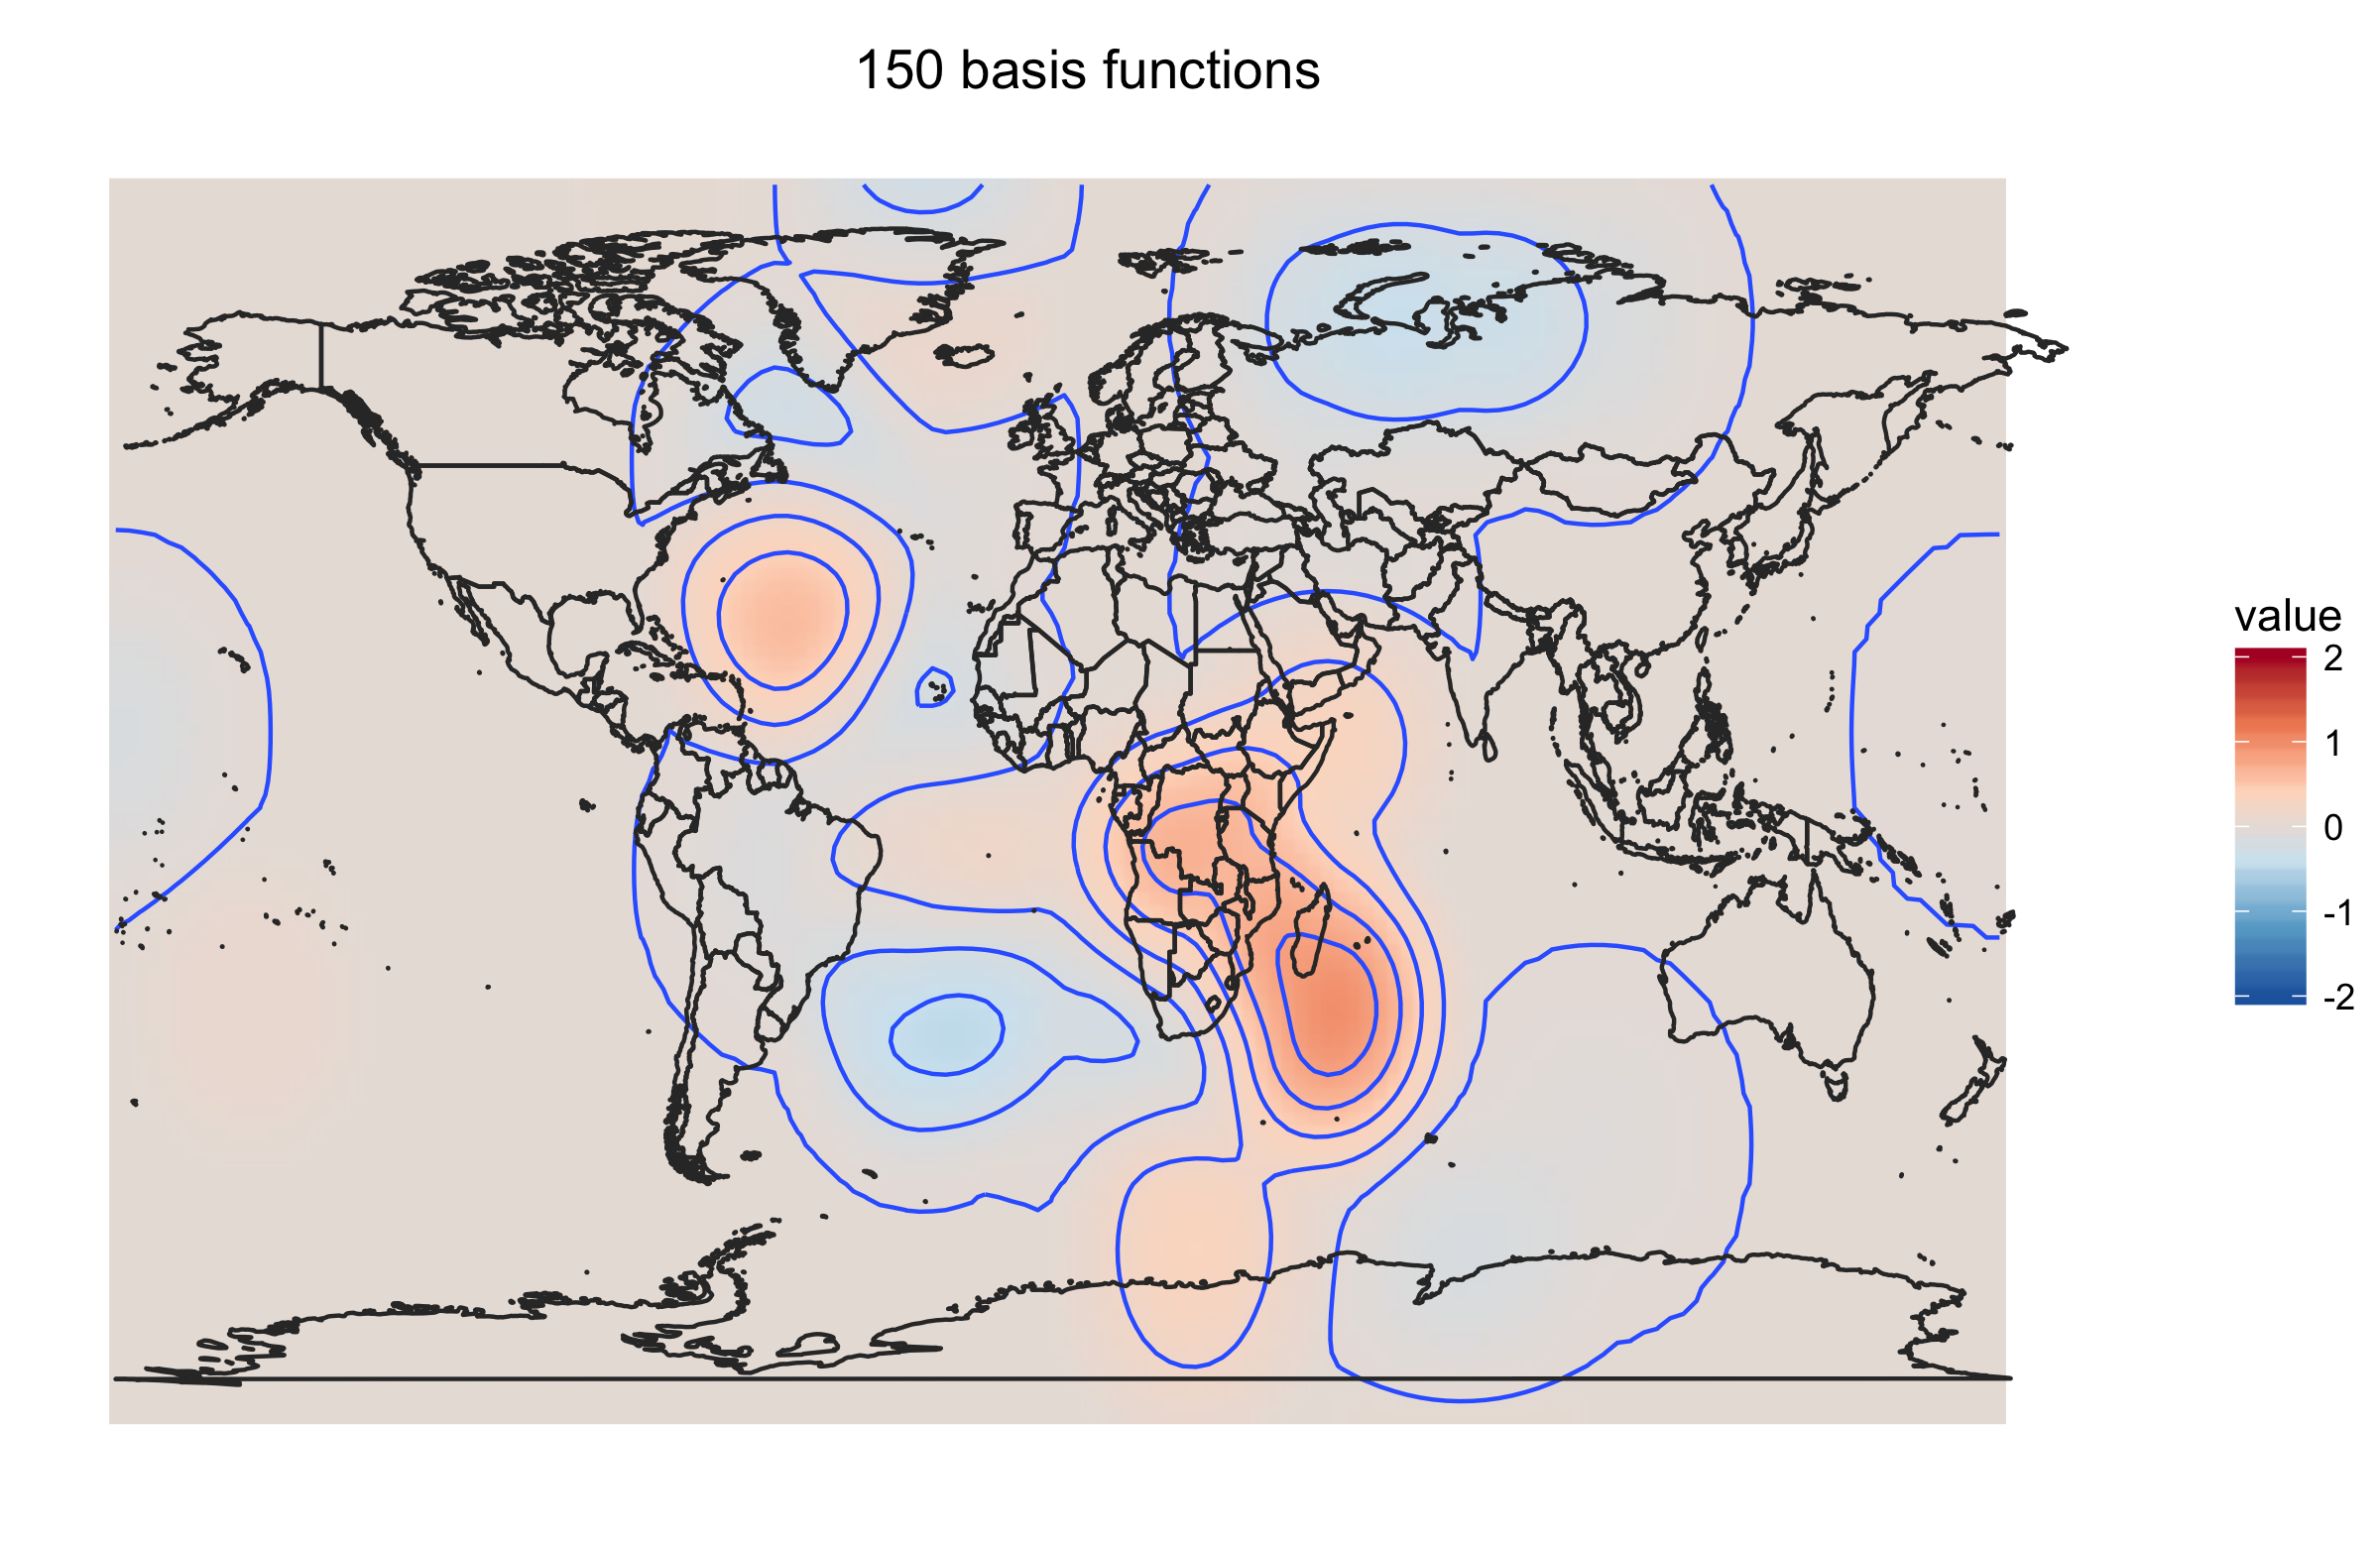
\includegraphics[width=0.7\textwidth,valign=c]{../plots/150coef.png}%
  }
  \subfloat{%
    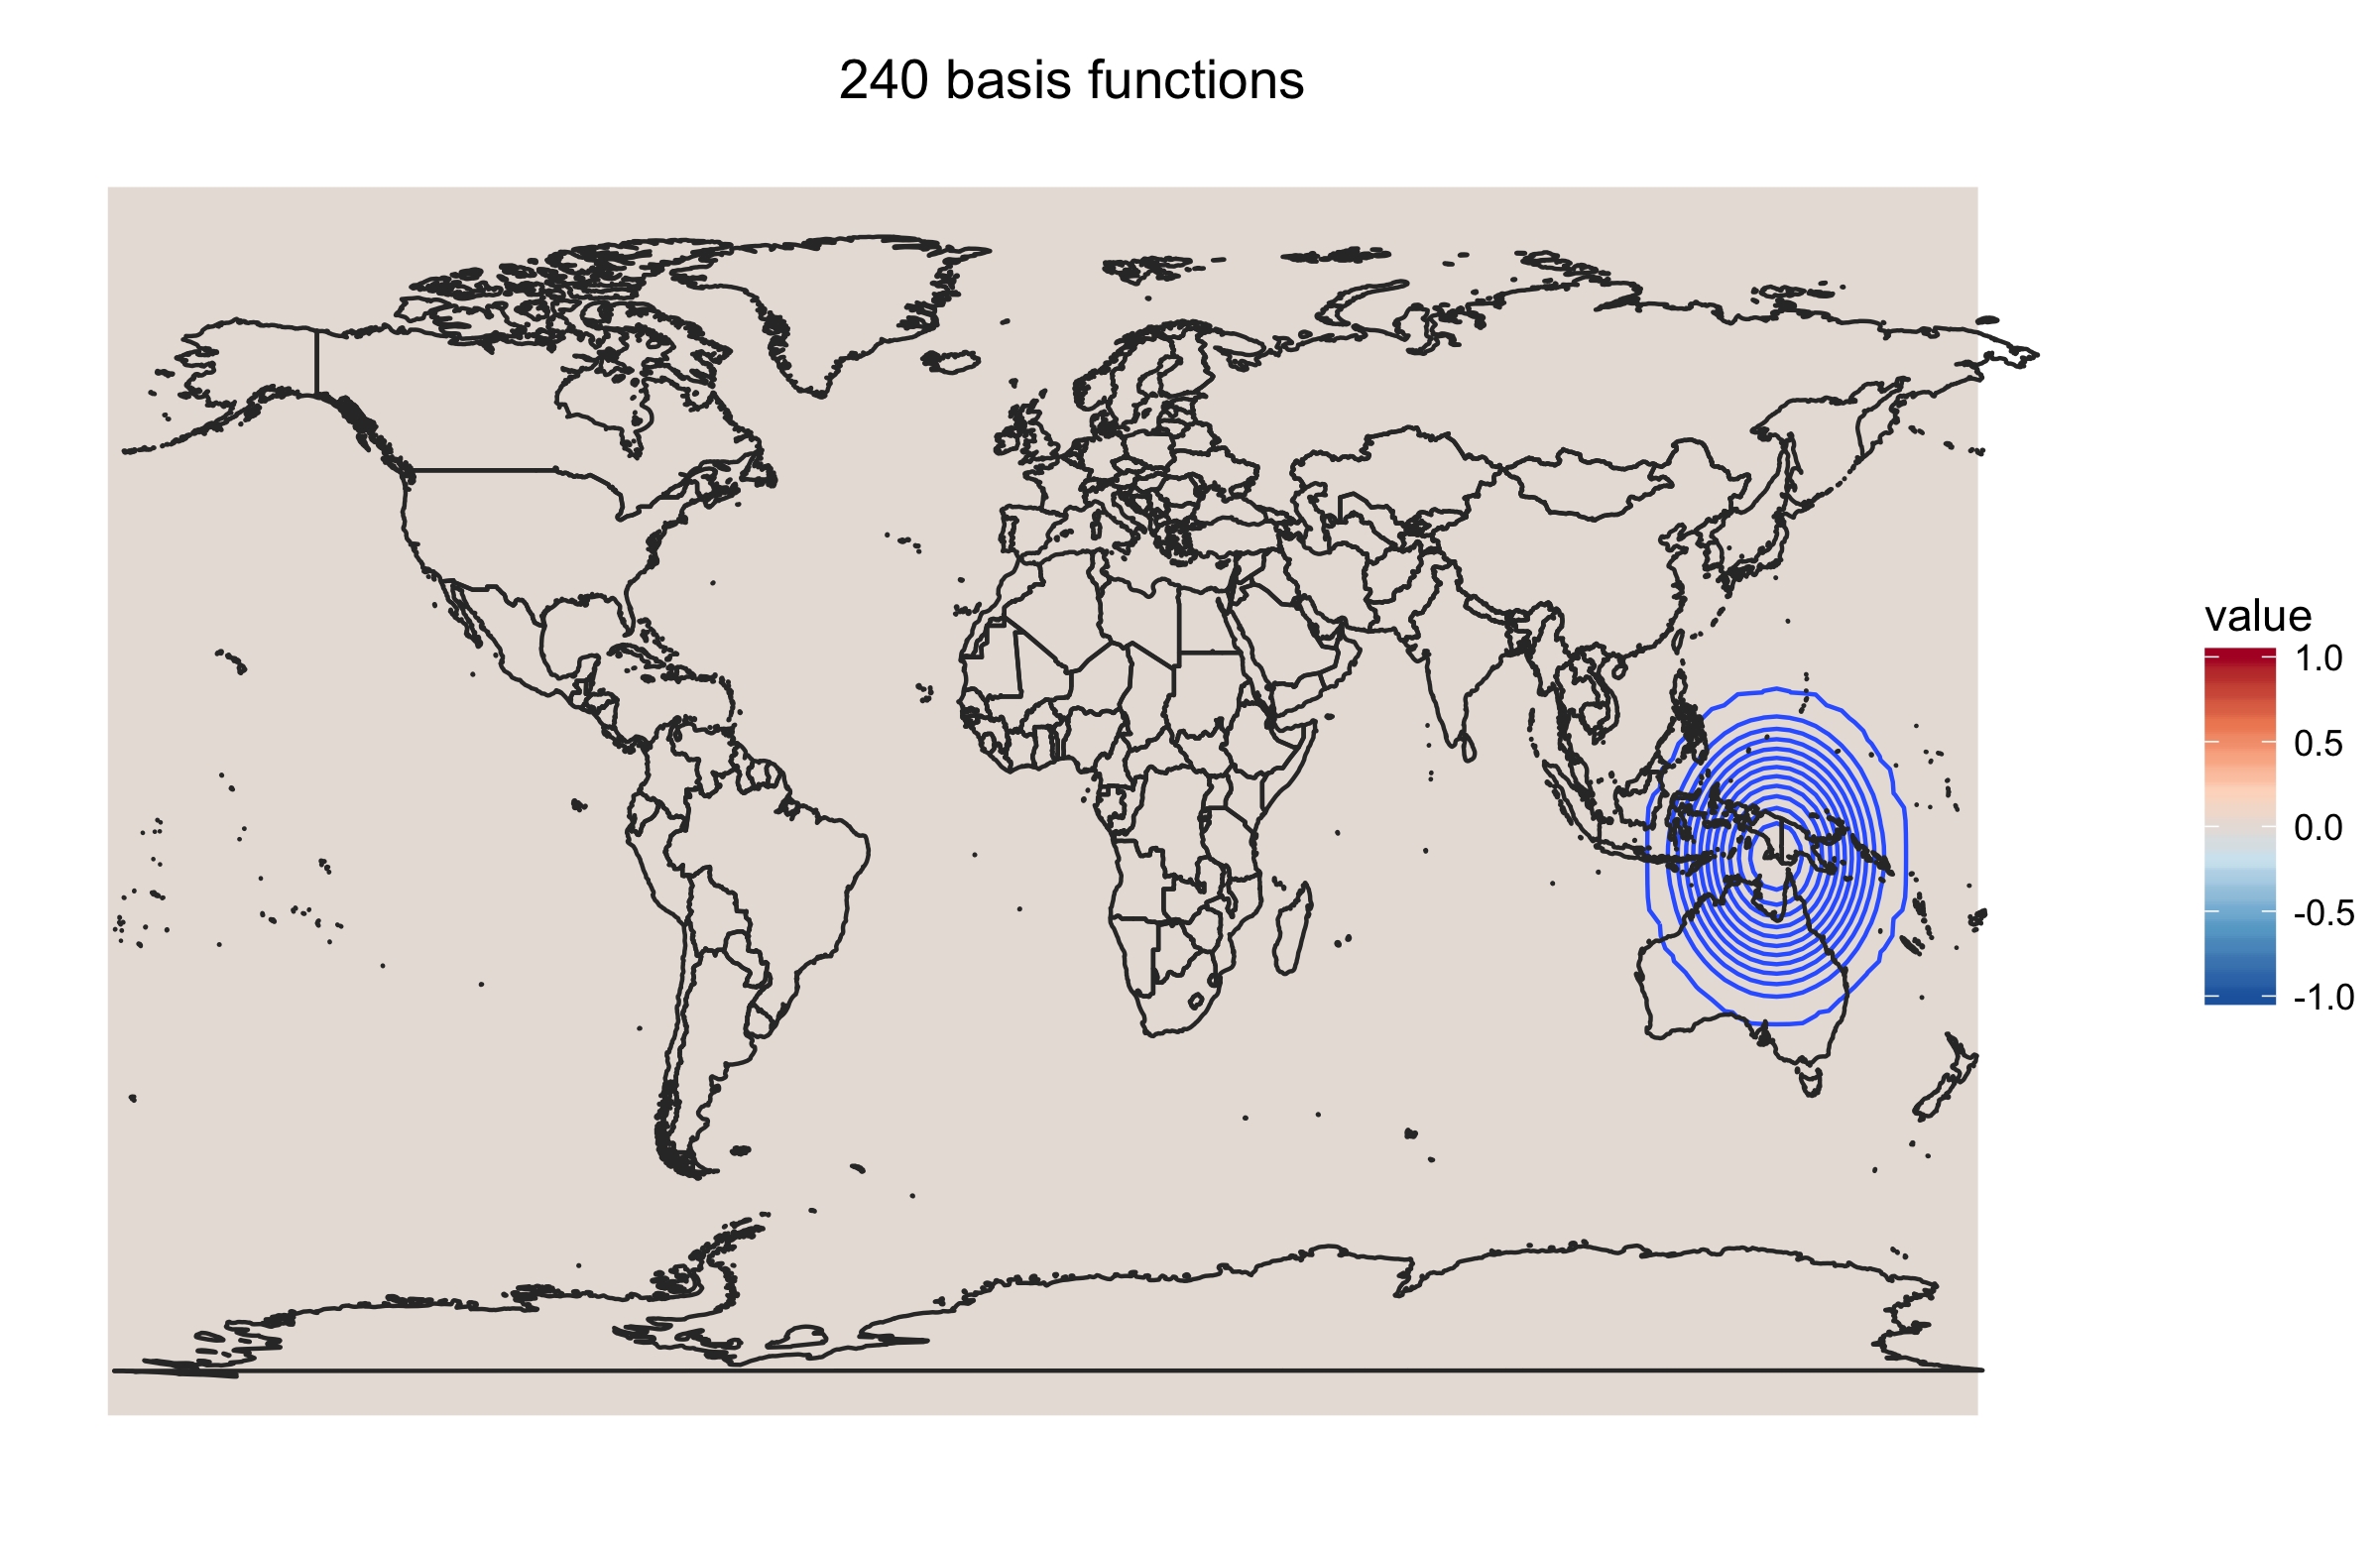
\includegraphics[width=0.7\textwidth,valign=c]{../plots/240coef.png}%
  }

  \hspace{-2.5cm}\subfloat{%
    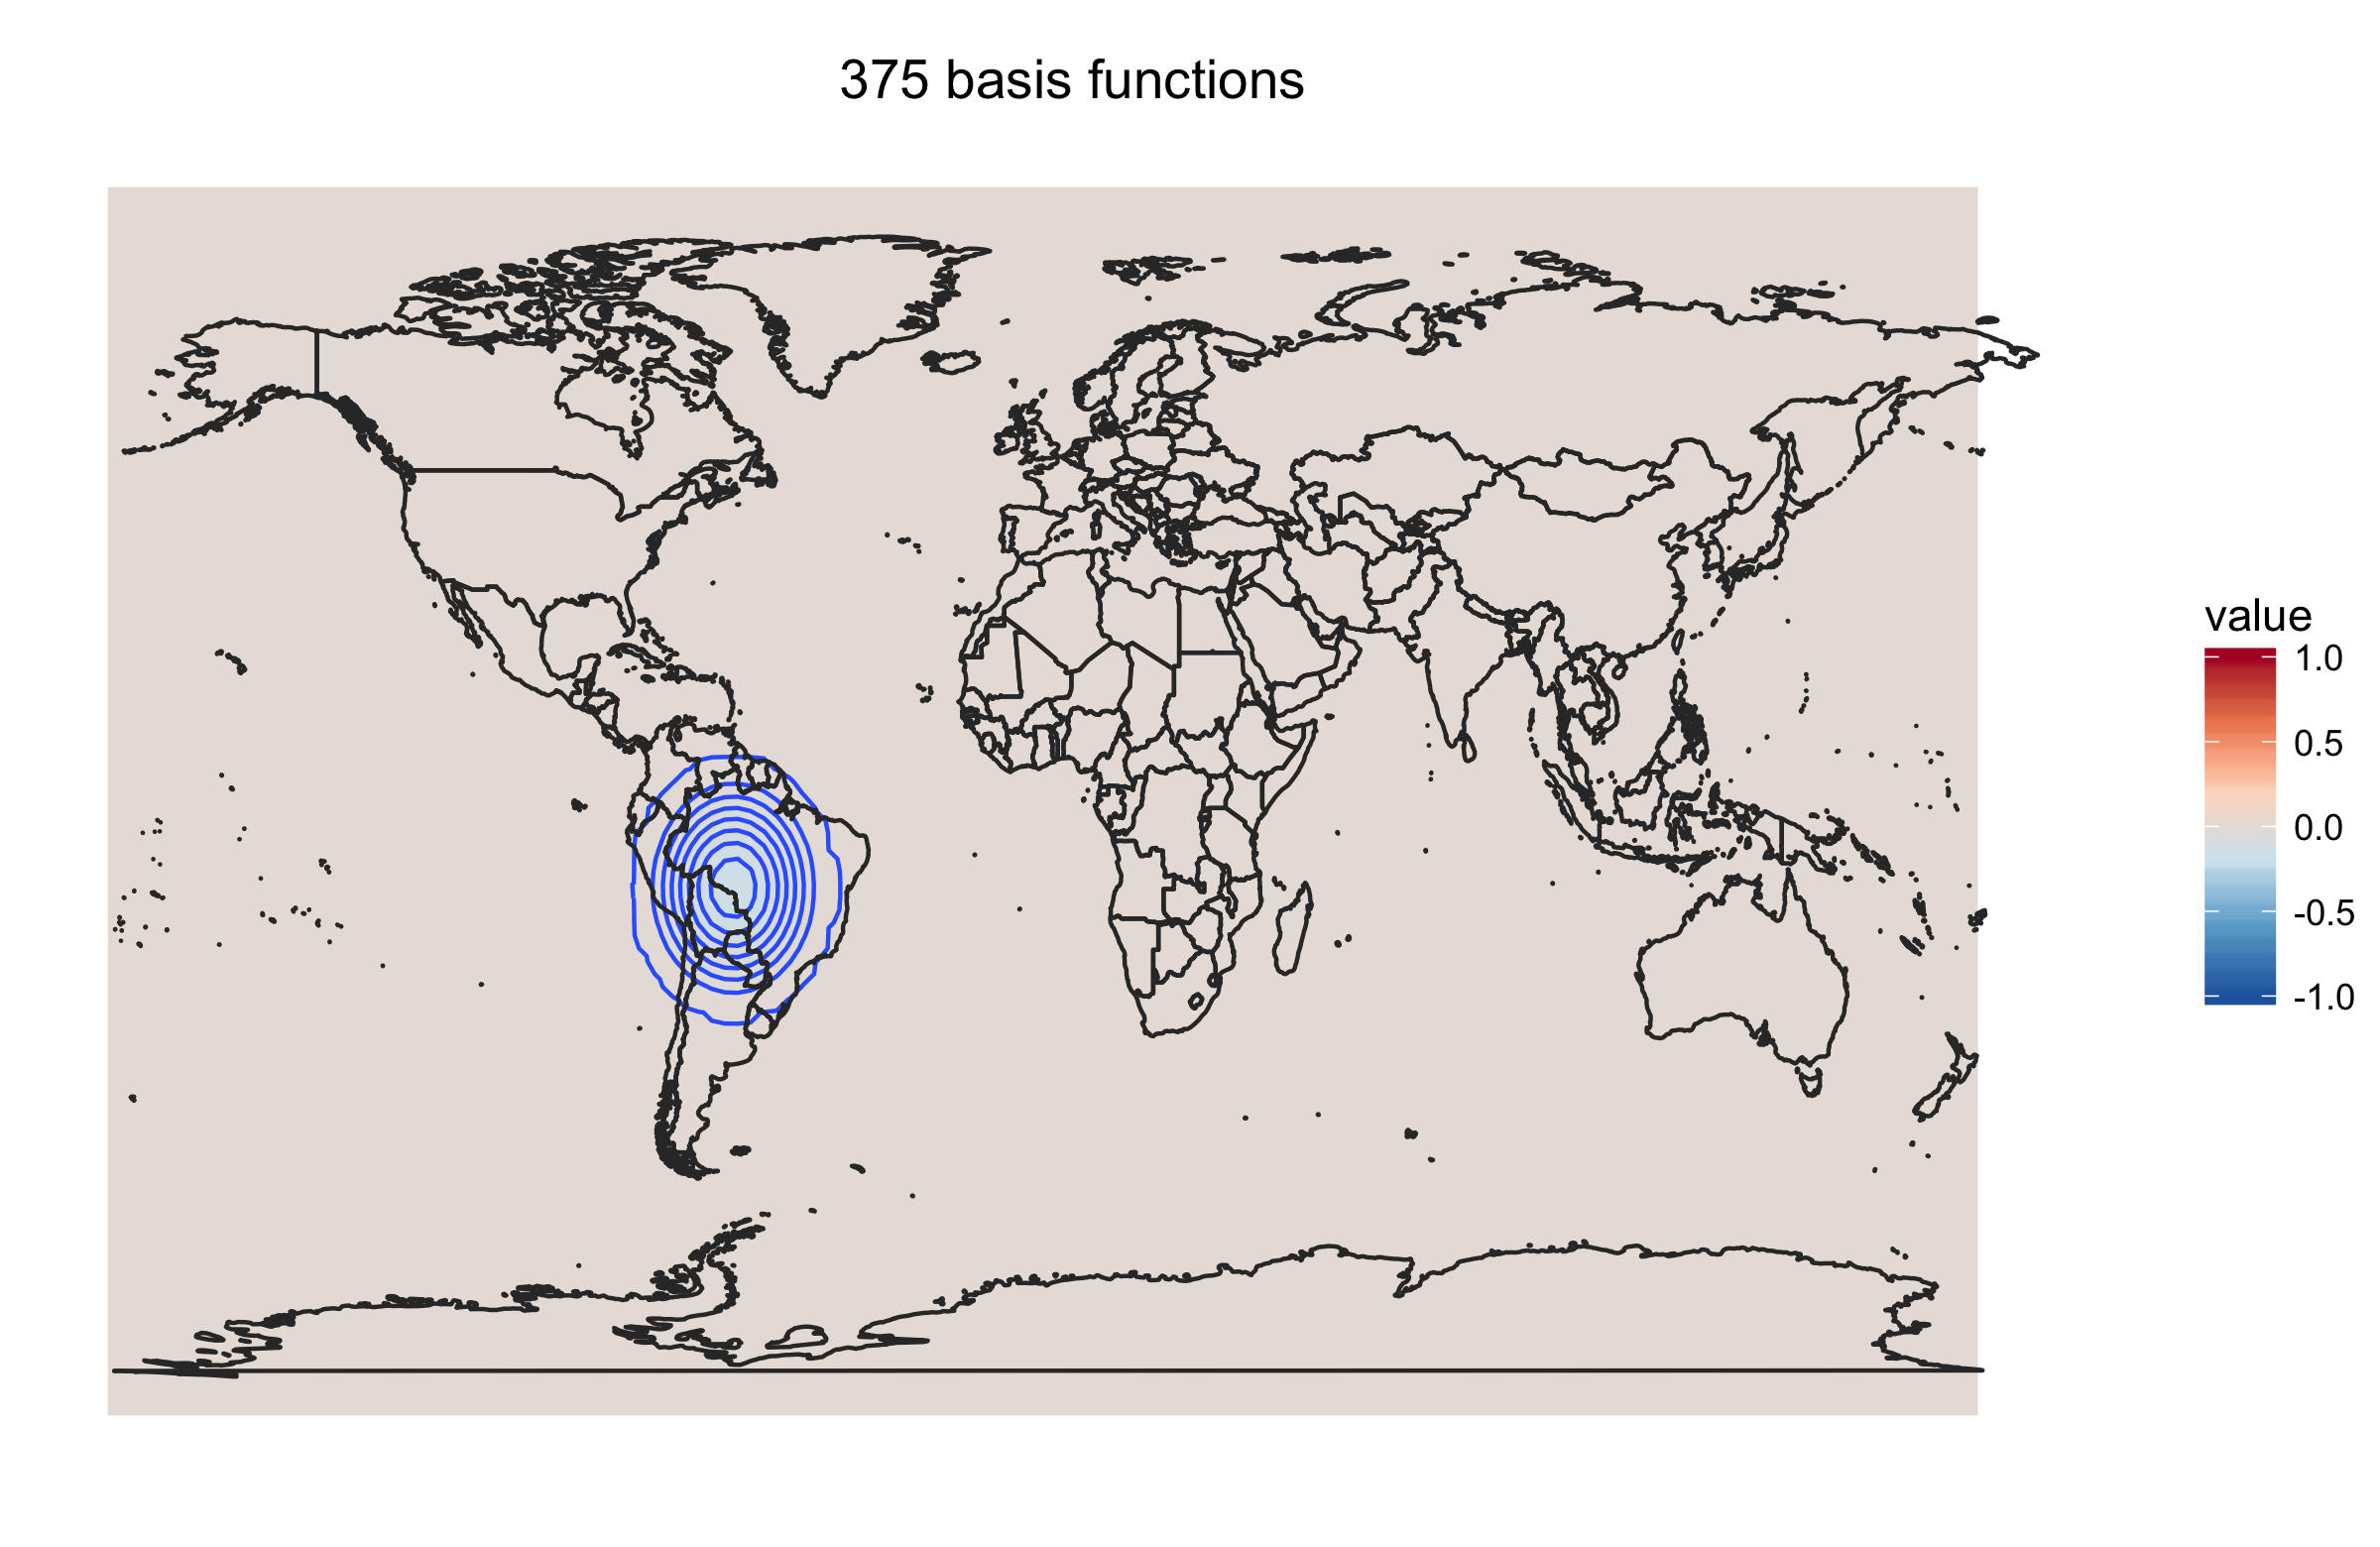
\includegraphics[width=0.7\textwidth,valign=c]{../plots/375coef.png}%
  } 
  \subfloat{%
    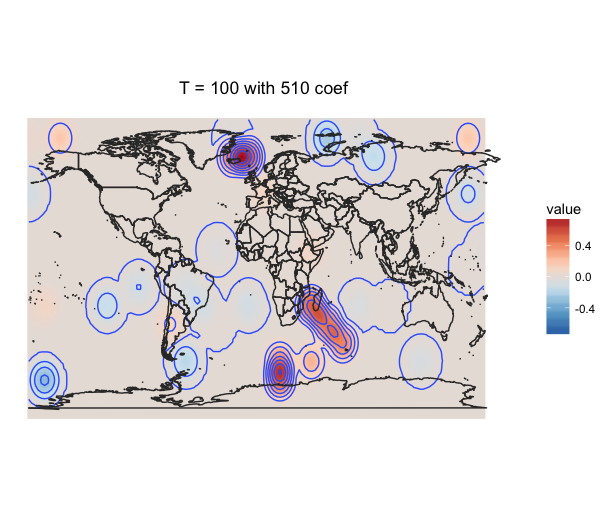
\includegraphics[width=0.7\textwidth,valign=c]{../plots/510coef.png}%
  }
  
\end{figure}


\subsection{Different time points}
Next, to see where and how the ensemble differs from the prior over time we plotted the difference fields at three widely separated time points. Since results are fairly dependent on the number of basis functions, all of these were constructed using 510 basis functions. The proxy network graph from Steiger (2018)\cite{steiger18} was also included since we suspected that differences may be most pronounced around proxy sites. At the three time points under consideration here this doesn't appear to be true though.

\begin{figure}[H]

  \hspace{-2.5cm}\subfloat{%
    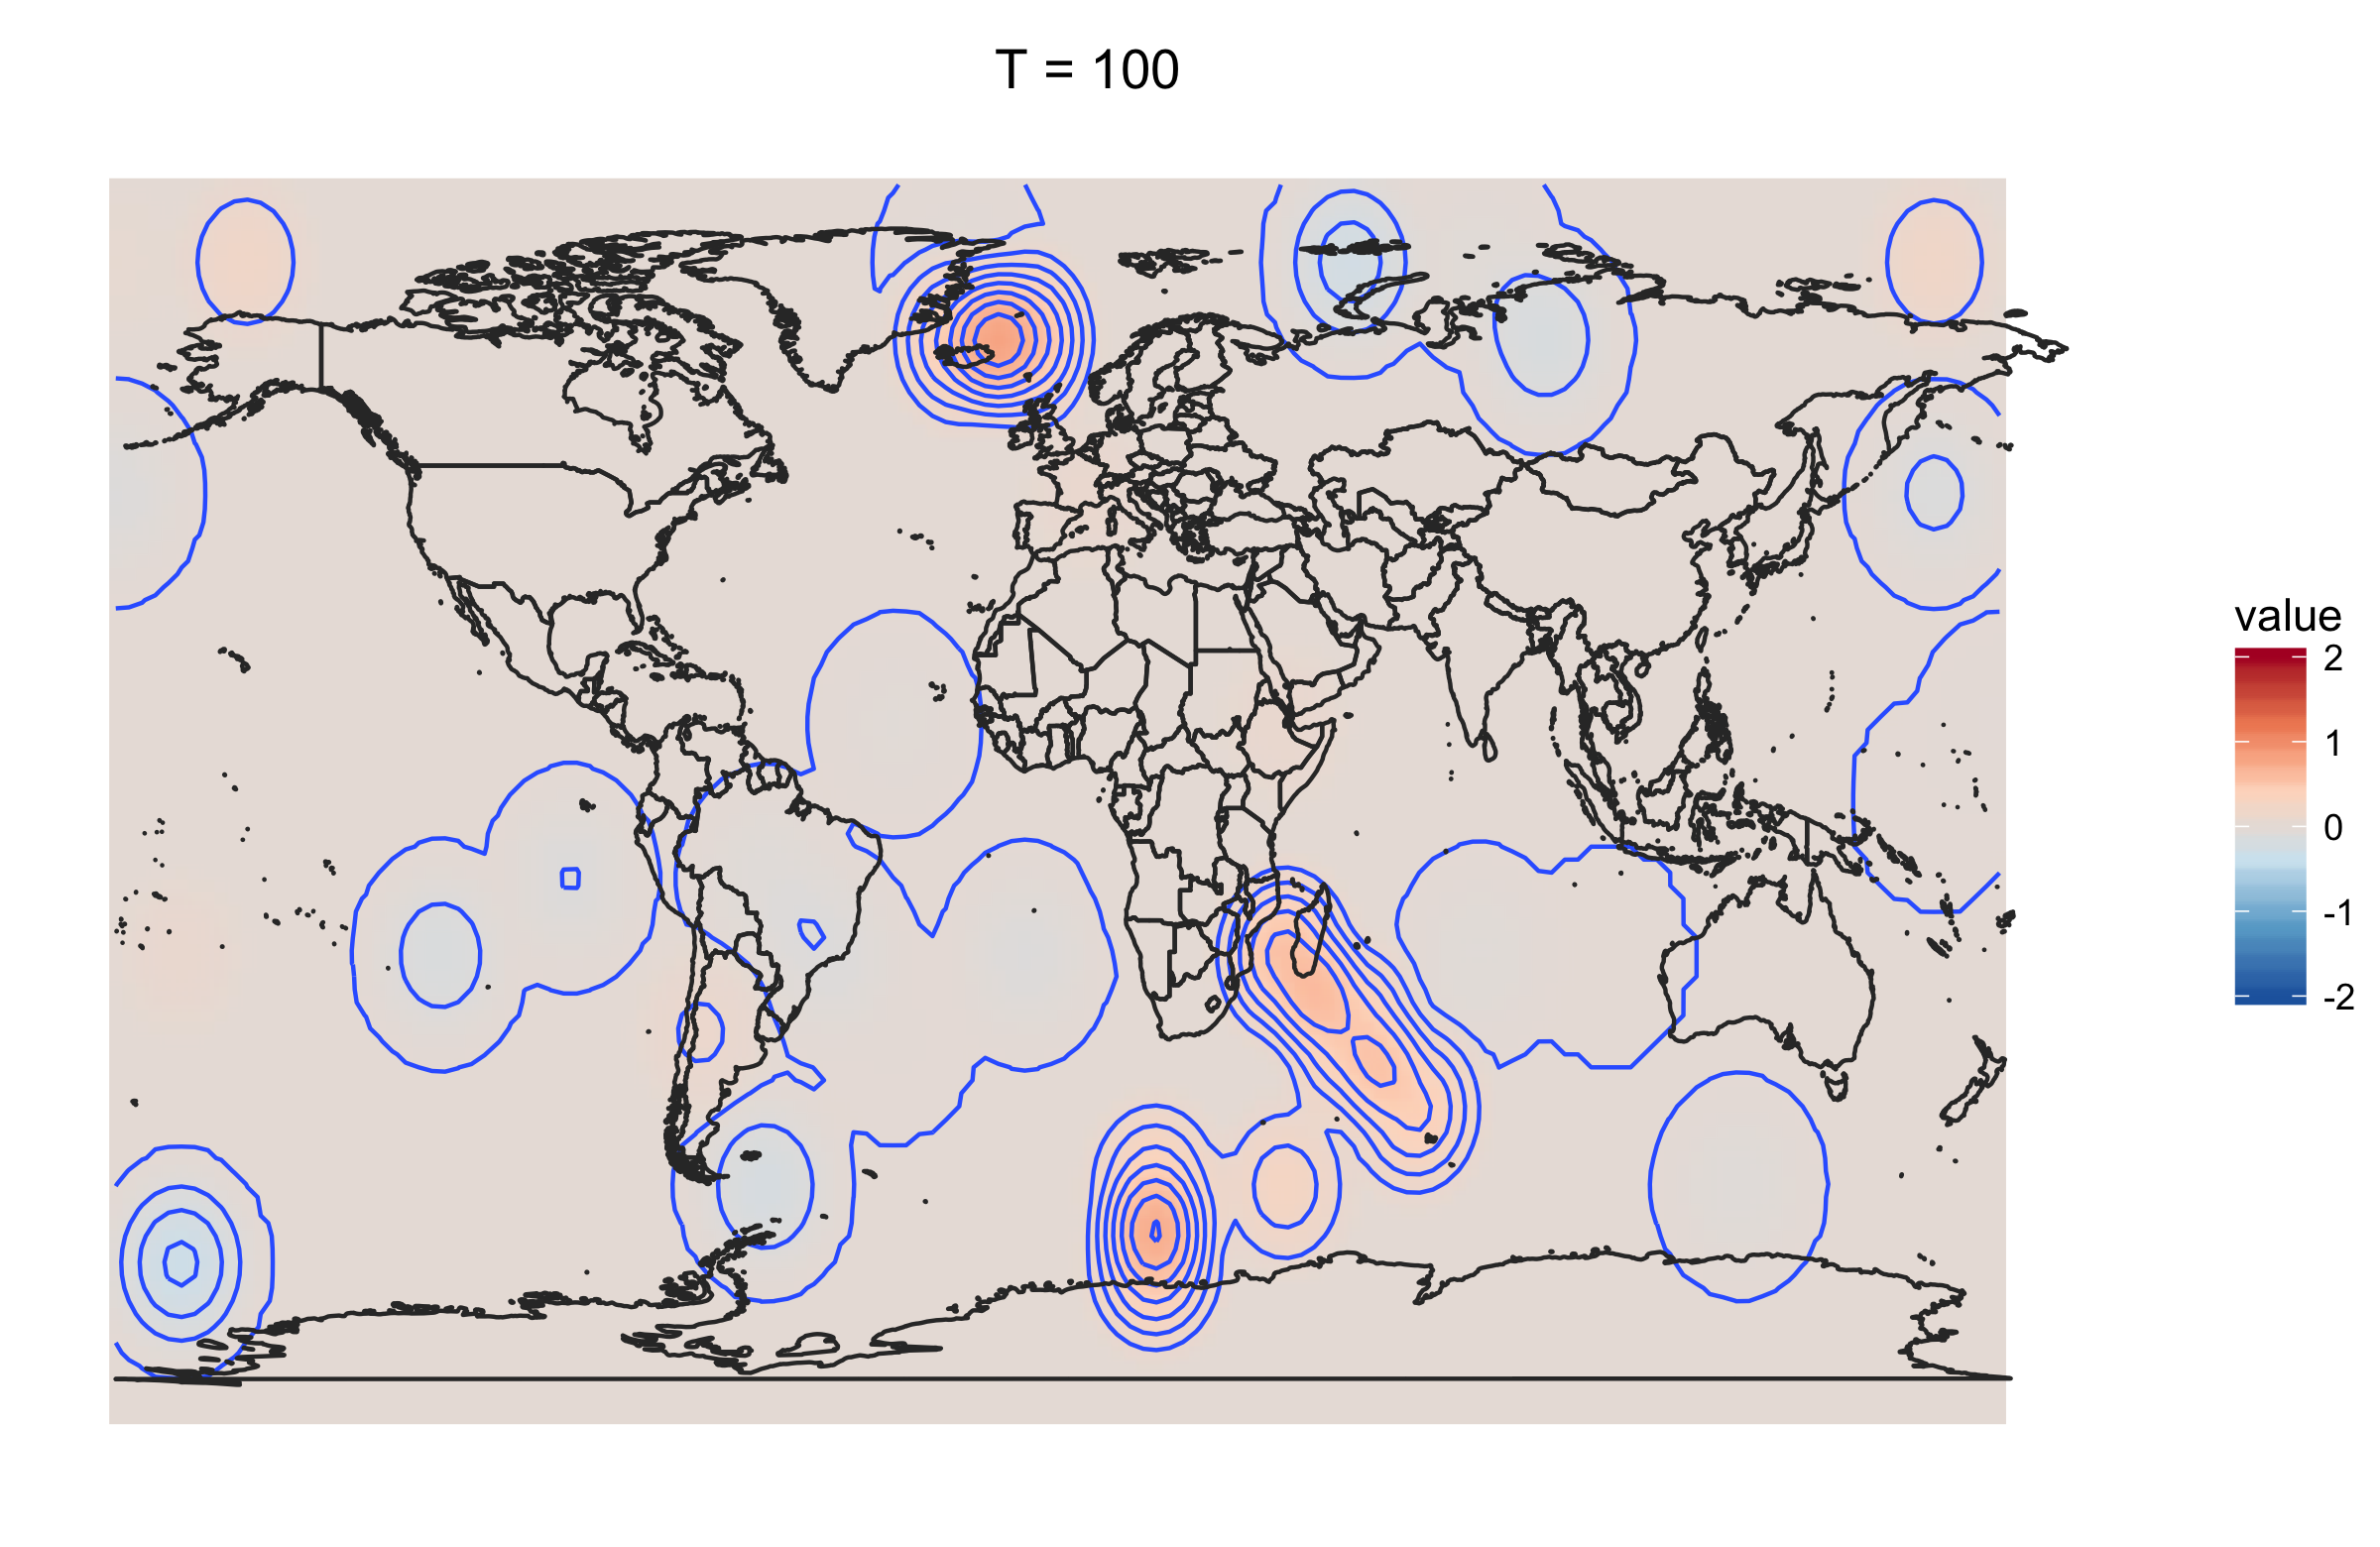
\includegraphics[width=0.7\textwidth,valign=c]{../plots/t100diff.png}%
  }
  \subfloat{%
    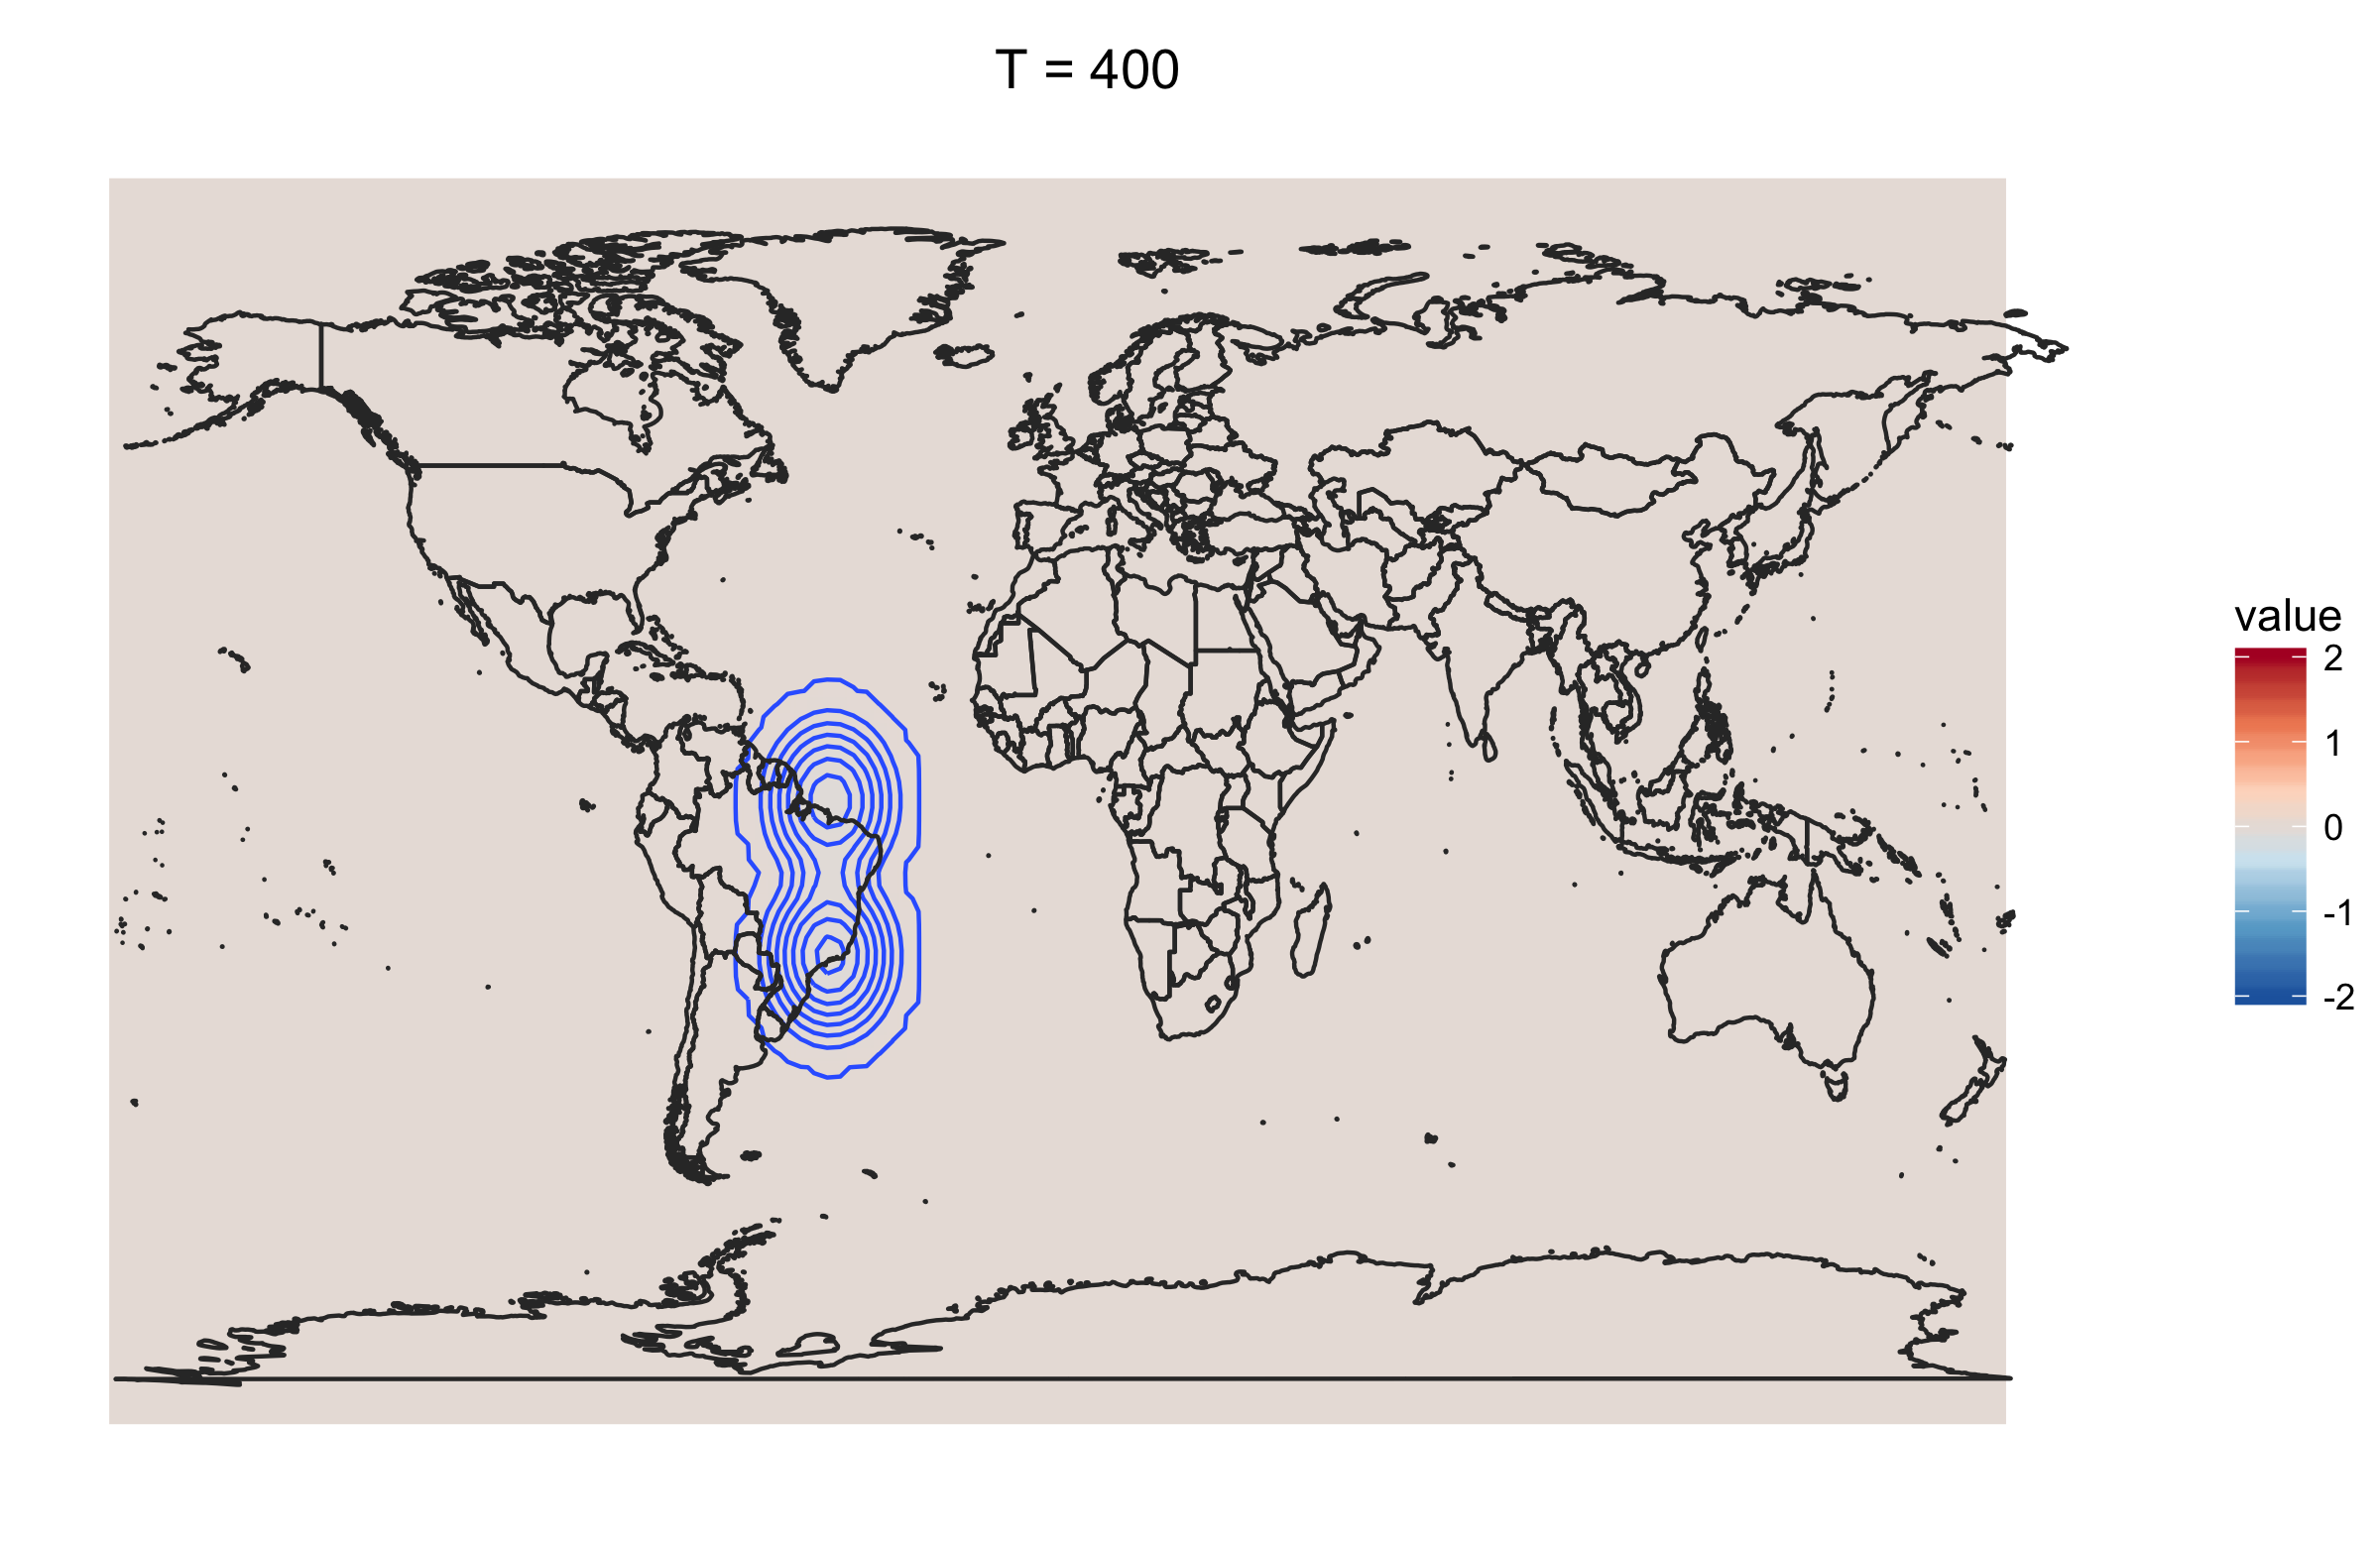
\includegraphics[width=0.7\textwidth,valign=c]{../plots/t400diff.png}%
  }

  \hspace{-2.5cm}\subfloat{%
    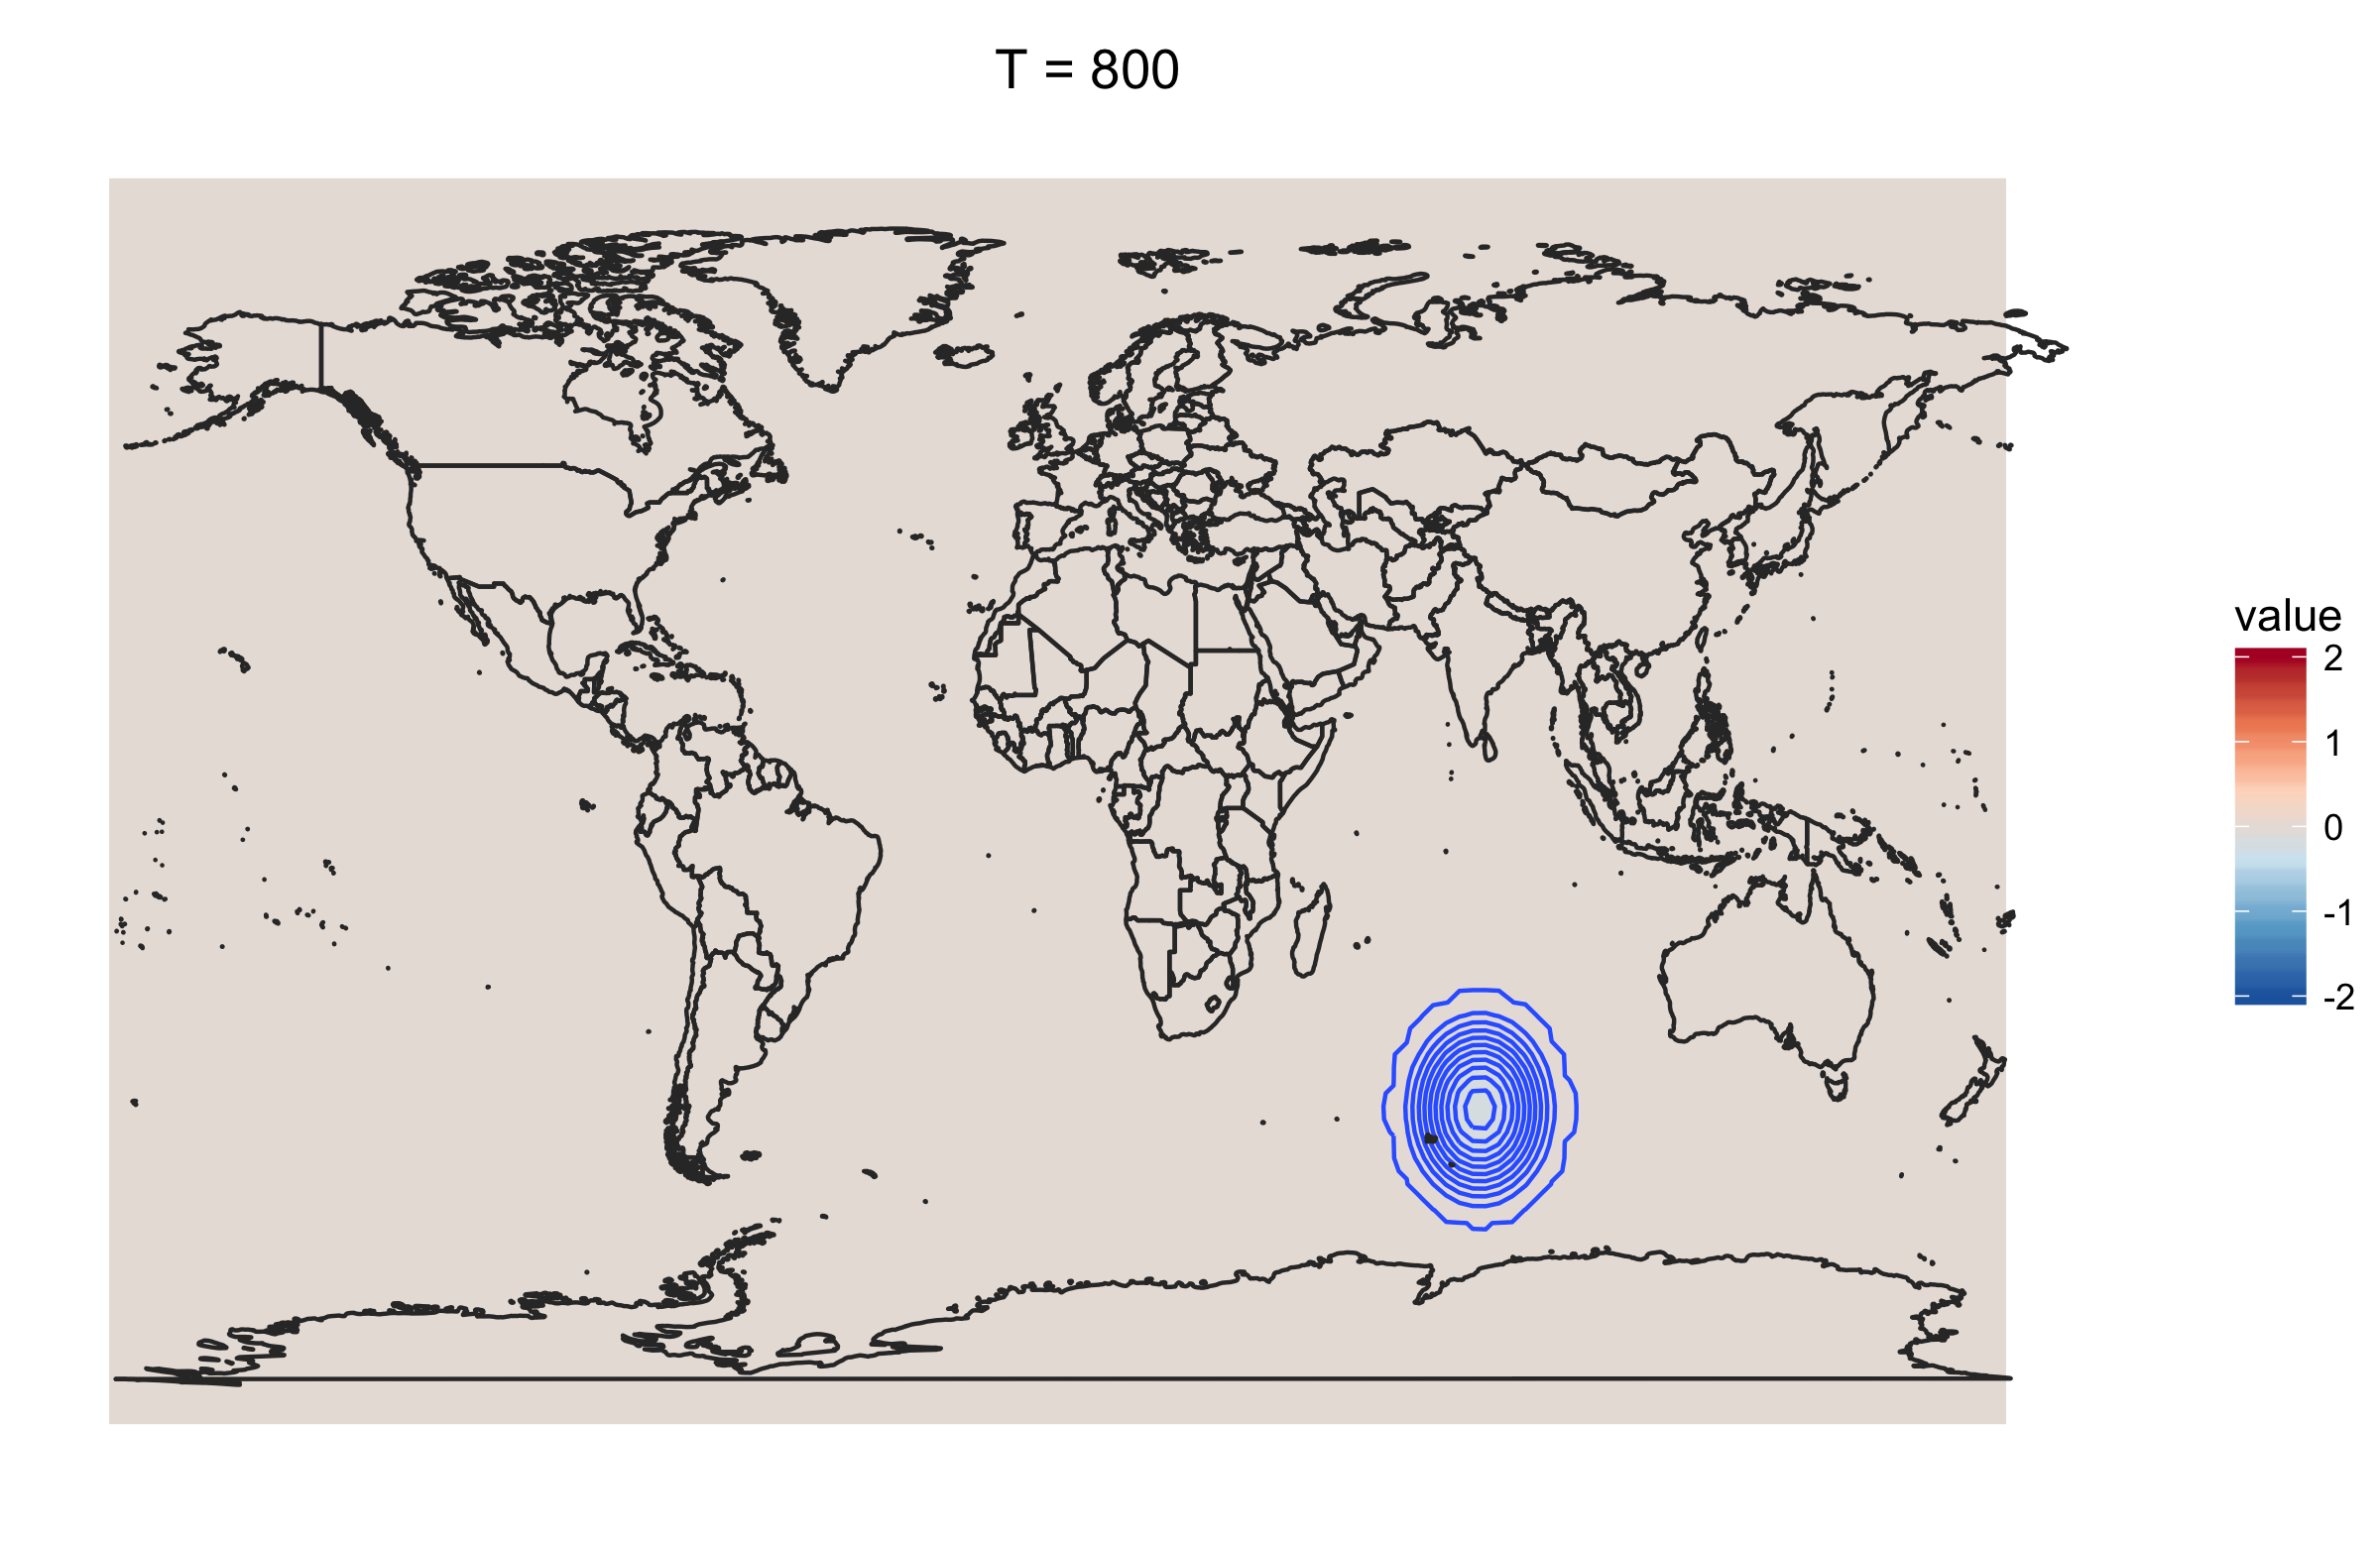
\includegraphics[width=0.7\textwidth,valign=c]{../plots/t800diff.png}%
  } 
  \subfloat{%
    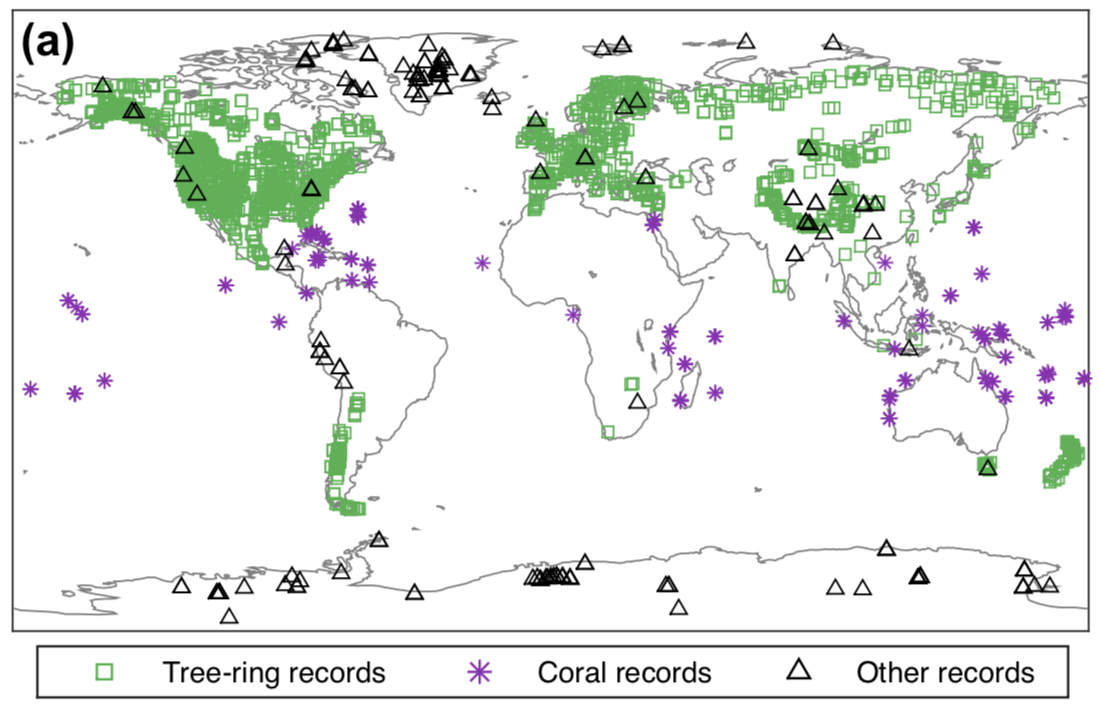
\includegraphics[width=0.6\textwidth,valign=c]{../plots/proxysites.png}%
  }
  
\end{figure}


\section{Conclusion}

\subsection{Summary}
Our intent for this phase of the project has been to test for and quantify differences between the prior and the ensemble. \sout{So far we have seen that at almost every time point ED registers the prior and the ensemble as being significantly different.} While these results may be the result of the information gain from the pseudo-proxies on the prior, some of this may be attributable to the fact that the representing basis coefficients tend to be very close together. This makes it fairly easy for the prior to test as being ``outside'' the range of the ensemble.

Furthermore, we have seen that where the prior and the posterior significantly differ can depend heavily on both time and the number of representing basis functions and that it is not necessarily tied to proxy locations.


\subsection{Questions}
\begin{enumerate}
	\item What further visualizations, statistics, etc would convey differences between the prior and the ensembles here? 
	\item Would a graph showing the average ``difference field'' over time be worth looking at? What about at specific time points?
	\item Are differences in some regions more important than others? And if so should an irregular or multi-resolution grid of basis functions be used instead? Alternatively we could replace OLS with a weighted version to stress these regions.
\end{enumerate}

\begin{thebibliography}{999}

\bibitem{cressie08}
	Cressie, Noel and Johannesson, Gardar (2008).
	``Fixed rank kriging for very large spatial data sets'',
	\textit{Journal of the Royal Statistical Society: Series B (Statistical Methodology)},
	70, 209-226
	
\bibitem{naveen15}
	Narisetty, Naveen and Nair, Vijayan (2015).
	``Extremal Depth for Functional Data and Applications'',
	\textit{Journal of the American Statistical Association},
	516, 1705-1714
	
\bibitem{Schwarz78}
	Schwarz, Gideon E (1978)
	``Estimating the dimension of a model'',
	\textit{Annals of Statistics},
	6 (2), 461–464
	
\bibitem{steiger18}
	Steiger, N.J., J.E. Smerdon, E.R. Cook, B.I. Cook, (2018)
	`` A reconstruction of global hydroclimate and dynamical variables over the Common Era.''
	\textit{In review}
\end{thebibliography}

\end{document}
